% ----- formatovani dokumentu -----------------------------------------------
\documentclass[12pt,a4paper,titlepage,final]{report}
\usepackage[utf8]{inputenc}
\usepackage[T1, IL2]{fontenc}
\usepackage{graphicx}
\usepackage{epstopdf}
\usepackage[margin=2cm]{caption}
\usepackage[top=3cm, left=2cm, right=2cm, text={17cm, 24cm}, ignorefoot]{geometry}
\usepackage{color}
\usepackage{url}
\usepackage{setspace}
\singlespacing
\usepackage[square, numbers]{natbib} 
\usepackage{float}
\pagestyle{plain}
\pagenumbering{arabic}
\setcounter{page}{1}
\setcounter{secnumdepth}{-1}
\setlength{\parindent}{1cm}	
\usepackage{natbib}
\usepackage{amsmath}
\usepackage{tocloft}
\usepackage{esvect}
\usepackage{amssymb}
\usepackage{gensymb}
\usepackage{subcaption}
\usepackage[algoruled,boxed,lined,longend]{algorithm2e}
\usepackage{mathtools}
\usepackage{listings}

\DeclareMathOperator{\dis}{d}

  \newenvironment{czechalgorithm}[1][htb]
  {\renewcommand{\algorithmcfname}{Algoritmus}% Update algorithm name
   \begin{algorithm}[#1]%
  }{\end{algorithm}}

% ----- vyberte jazyk -------------------------------------------------------
\usepackage[english]{babel}
%\usepackage[english]{babel}

% ----- dopiste titulky -----------------------------------------------------
\newcommand\Course{Visualization \& CAD}
\newcommand\WorkTitle{Outrun scene with a car}
\newcommand\Author{Petr Flajšingr}
\newcommand\AuthorEmail{xflajs00@stud.fit.vutbr.cz}
\newcommand\Faculty{Faculty of Information Technology}
\newcommand\School{Brno University of Technology}

\usepackage[
pdftitle={\WorkTitle},
pdfauthor={\Author}
bookmarks=true,
colorlinks=true,
breaklinks=true,
urlcolor=blue,
citecolor=blue,
linkcolor=blue,
unicode=true,
]
{hyperref}


% ----- titulni strana ------------------------------------------------------

\begin{document}
	\begin{titlepage}
	\begin{center}
		\begin{Large}
			\Course\\
		\end{Large}
		\bigskip
		\begin{Huge}
			\WorkTitle\\
		\end{Huge}
	\end{center}
	\vfill
	\begin{center}
		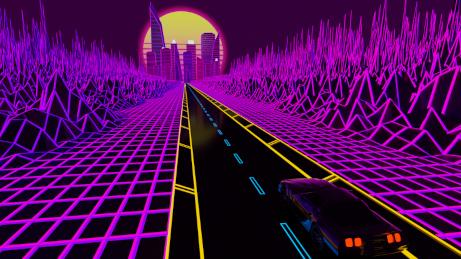
\includegraphics[height=10cm]{images/render_small.png}
	\end{center}
	\vfill
	\begin{center}
		\begin{large}
			\today
		\end{large}
	\end{center}
	\vfill
	\begin{flushleft}
		\begin{large}
			\begin{tabular}{lll}
				Author: & \Author, & \url{\AuthorEmail} \\
				& \Faculty \\
				& \School \\
			\end{tabular}
		\end{large}
	\end{flushleft}
\end{titlepage}		

\tableofcontents
\newpage

\section{Introduction}
The aim of this project is to create an outrun scene using Blender along with a simple animation created on this scene. All of the models in the scene were created in blender and the animation was created using Blender's animation functions. Rendering is done via path tracing, thanks to which there are reflections in the scene - this enhances the desired aesthetic of the scene greatly.

\section{Theoretical foundations}
\subsection{Subdivision modeling}
Subdivision modeling is one of the most popular techniques form 3D modeling. It provides capabilities to create models which are easily scalable and look good when rendered. This method is based around how the models are rendered in most of cases - polygons. 

First lets define some terminology which is necessary for understanding this method:

\begin{itemize}
    \item \textbf{Vertex} -- a point in space which serves as a coordinates of edge's start/end.
    \item \textbf{Edge} -- a connection between two vertices.
    \item \textbf{Polygon} -- a face of a 3D shape, which connects several vertices via edges.
    \item \textbf{Mesh} -- a collection of polygons which are combined to create a shape in 3D space. May be referred to as a model or a body.
    \item \textbf{Triangle} -- a polygon with 3 vertices and 3 edges.
    \item \textbf{Quad} -- a polygon with 4 vertices and 4 edges.
    \item \textbf{N-Gon} -- a polygon with N vertices and N edges.
    \item \textbf{Pole} -- a vertex with 3 edges coming out of it.
    \item \textbf{N-Pole} -- a vertex with N edges coming out of it.
\end{itemize}

In other words a 3D shape can be called mesh, model or body. It is constructed from polygons which are made from edges and these edges are situated between vertices. 

\begin{figure}[H]
    \centering
    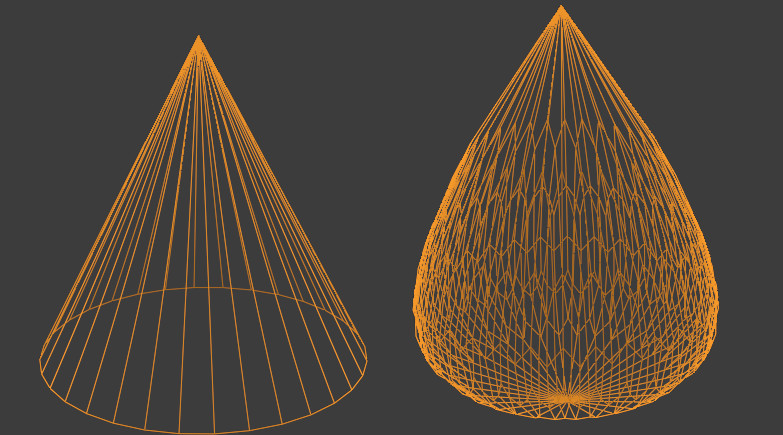
\includegraphics{images/subdiv.jpg}
    \caption{Example of subdivision}
    \label{fig:subdivision}
\end{figure}

Subdivision comes into play when we want to smooth out the mesh. A raw mesh may have issues with overly sharp edges that distort the look of a model. It aims to divide the mesh into more polygons and vertices, while still maintaning the semblance of the original -- for example a quad would be divided into 4 quads, creating a new vertex and midpoint of the original 4 vertices. \cite{subdivision}

An example of subdivision algorithm is Catmull-Clark, which is used in Blender for example. It defines its surfaces recursively. For each mesh of a face a \textit{face point} is added. For each edge and \textit{edge point} is added. Then for each vertex an average is taken of all face points, which are touching the vertex and a new face is created. This can be repeated N times to further subdivide the surface. \cite{CATMULL1978350}

\begin{figure}[H]
    \centering
    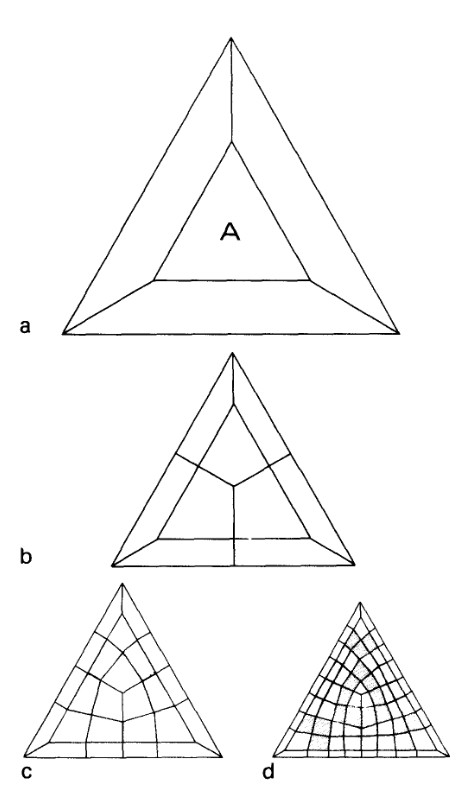
\includegraphics{images/subdiv_clark.jpg}
    \caption{Catmull-Clark subdivision \cite{CATMULL1978350}}
    \label{fig:cat_clark_subdiv}
\end{figure}


\subsection{T-splines}
A mathematical model for defining 3D surfaces based on NURBS surface. The model consists of control grid which contains control points. These points are connected by t-edges and each of these edges is constrained. Unlike some other models it allows for T-junctions, which allows for lower amount of control points and makes the modeling process easier. \cite{sederberg_zheng_bakenov_nasri_2003}

\begin{figure}[H]
    \centering
    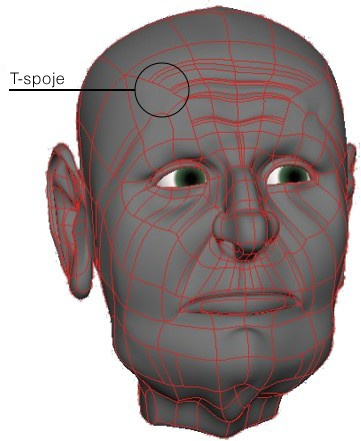
\includegraphics{images/tsplines.jpg}
    \caption{T-spline model \cite{tsplines}}
    \label{fig:tsplines}
\end{figure}

\subsection{Textures}
Textures are images, which can be applied to surfaces of 3D models \cite{wang}. There are many types of extures, some of those are:

\begin{itemize}
    \item Albedo - usually RGB textures, which are mapped onto a mesh. These provide surface's color.
    \item Normals - these textures are used to modify surface normal at a given point to provide an illusion of 3D texture on a surface.
    \item Parallax - textures similar to normal textures, although these can affect the surface in a way which provides much more detail without the need to have an insane amount of polygons. 
    \item Roughness - defines how light is scattared across the surface of a model. 
    \item Specular - defines how reflective the surface is.
    \item Metalness - very similiar to roughness, it is used to simulate metalic materials.
\end{itemize}

Textures may be generated proceduraly as well. This method is often used on water surfaces for both the color and normals. Common source of procedural textures are noise functions - perlin noise for example.

\begin{figure}[H]
    \centering
    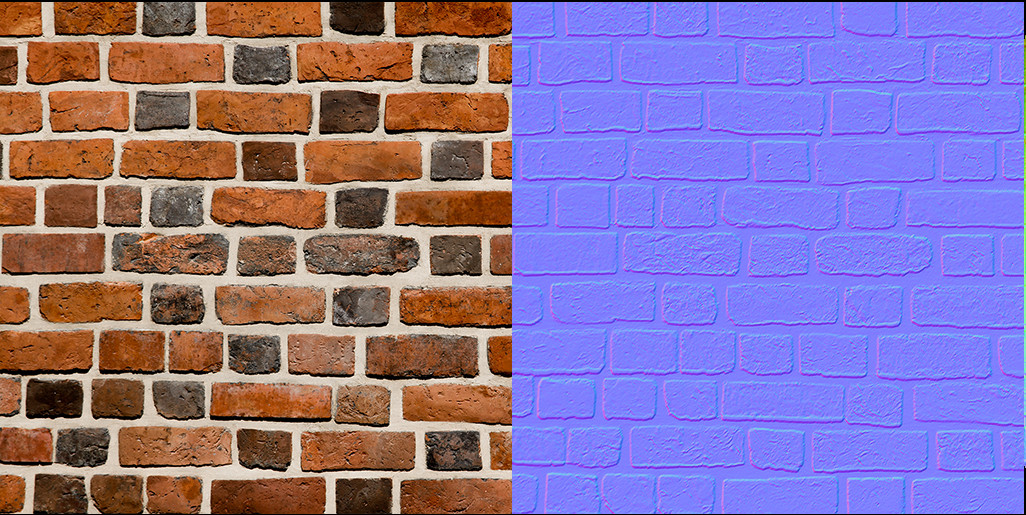
\includegraphics{images/textures.jpg}
    \caption{Albedo texture and normals texture \cite{wikipedia_2021}}
    \label{fig:cat_clark_subdiv}
\end{figure}

Textures are mapped via UV coordinates, which wrap the texture on the surface of a mesh. These coordinates are usually a part of the mesh itself, although they can be generated procedurally as well. Concerning the procedural mapping of textures, there are many types, some examples are on figure \ref{fig:mapping}.

\begin{figure}[H]
    \centering
    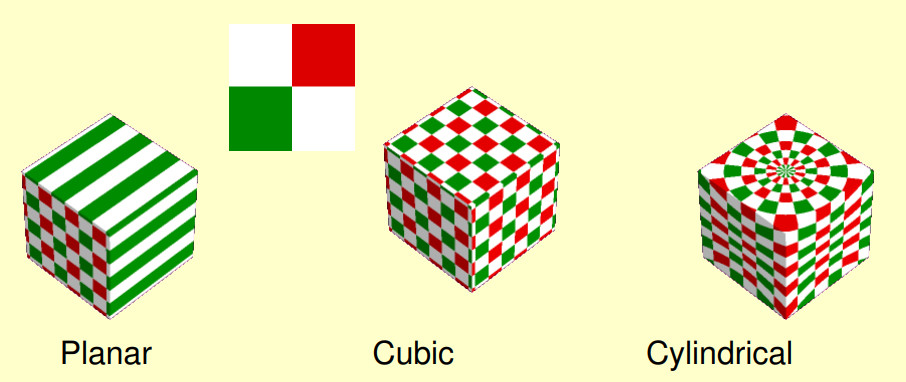
\includegraphics{images/mapping.jpg}
    \caption{Examples of texture mapping \cite{mapping}}
    \label{fig:mapping}
\end{figure}


\section{Motivation}
My motivation for creating this project is to learn atleast basics of 3D modeling, since it may be useful to me in my future practice. Theme of the scene was selected purely due to my personal preferences.

\section{Used tools}
The entire project was created in Blender 2.92 \footnote{\url{https://www.blender.org/}} - a software for creation of 3D models/scenes, motion graphics, simulations etc.. No other tools were used.

\section{Workflow description}
The first part of the project to be created was a model of a car. Before beginning modeling a blueprint for the model needs to be selected. I chose a blueprint of Corvette C4, since it fits nicely into the 80s era. The blueprints must be added to Blender as background images as shown on figure \ref{fig:blueprints}. The blueprint was downloaded from \url{https://the-blueprints.com/}.

\begin{figure}[H]
    \centering
    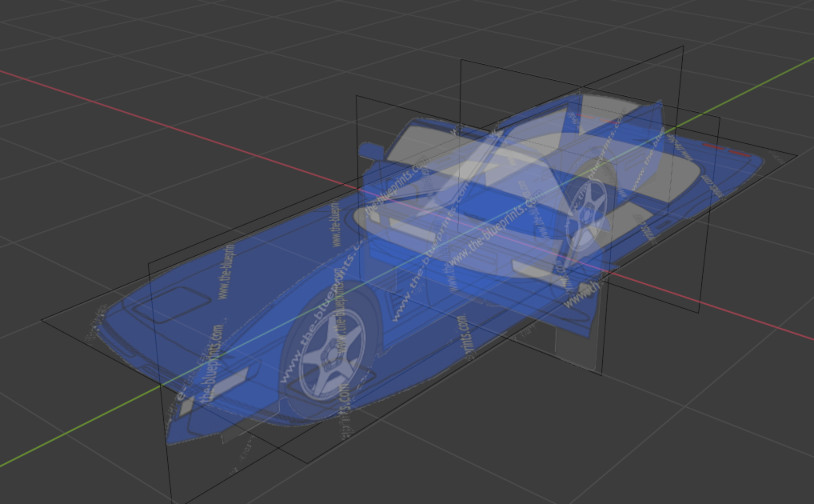
\includegraphics{images/blueprints.jpg}
    \caption{Blueprints}
    \label{fig:blueprints}
\end{figure}

After preparing blueprints i started modeling with a simple plane. I applied several modifiers to it to simplify the overall process:
\begin{itemize}
    \item Mirror - no need to create both sides, which should be the same either way.
    \item Soldify - nicely approximates width of the body.
    \item Subdivision surface - for easier operation while subdividng the surface.
\end{itemize}

Next i started subdividing and modifying the plane in order to fit the car outline. I divided the car into several parts to make the process easier - front part of the body \& roof, trunk, doors and windows. 

\begin{figure}[H]
    \centering
    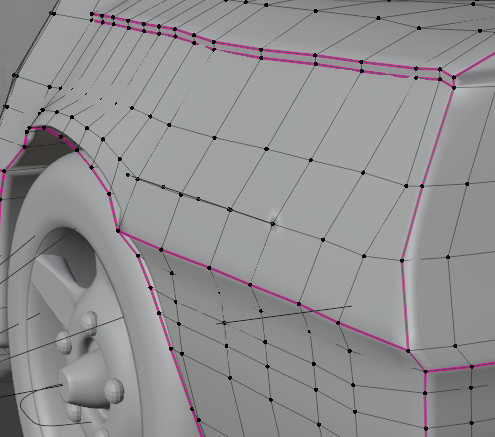
\includegraphics{images/edge_crease.jpg}
    \caption{Modeling detail}
    \label{fig:edge_crease}
\end{figure}

Due to the use of soldify i had to use edge crease function (marked pink in figure \ref{fig:edge_crease}) to create sharp edges on the model. Otherwise the entire process is just trying to match the outline provided by blueprints as close as possible.

A separate part of the car are its wheels. These were modeled separately and the process is a bit different. The wheel itself can be considired to be made by two separate pieces - rim and tire. Let's focus on the rim first.

Modeling of the rim can be greatly simplified, because it's a symetrical object. I created a circle, extruded it and selected every second face on the outer side using checker deselect. After that all parts were modeled simultaneously. The outer part is again simply extruded circle. The entire object has Subdivision surface modifier applied to it.

\begin{figure}[H]
    \centering
    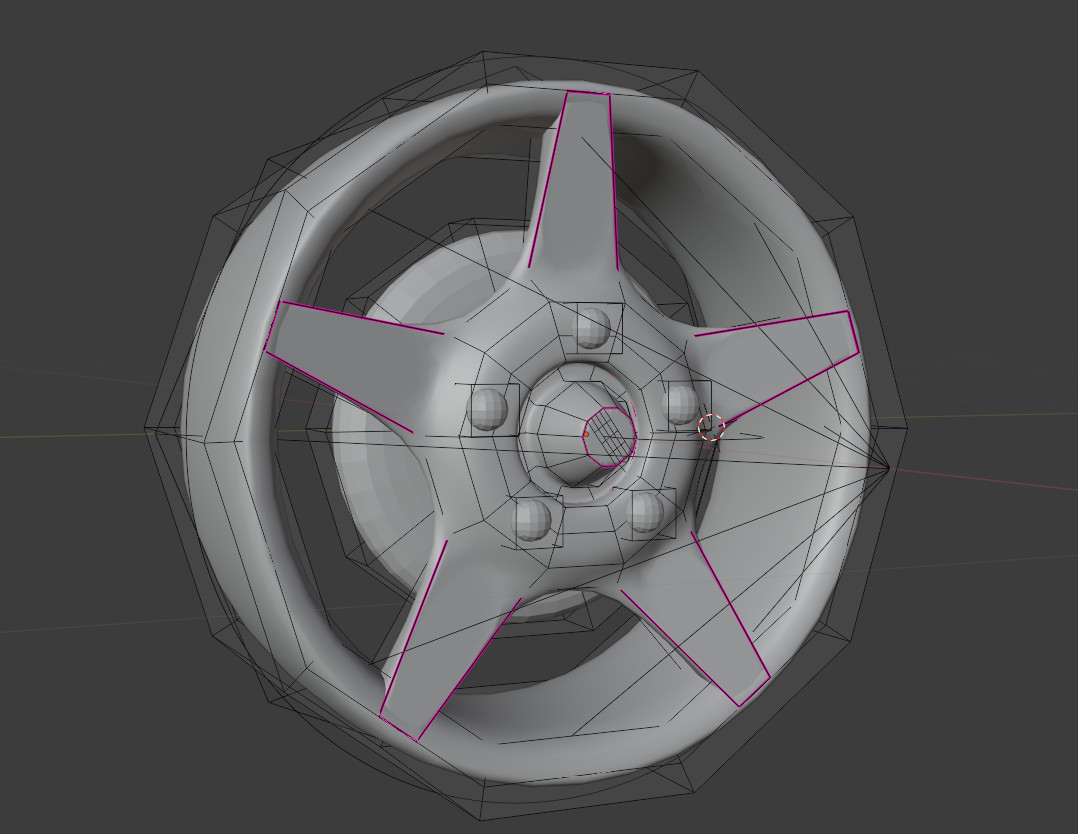
\includegraphics{images/rim.jpg}
    \caption{Modeling rim}
    \label{fig:rim}
\end{figure}

Tires require a bit different process. Modeling it polygon by polygon would be tedious. I started with a blueprint of a real-world tire to copy its pattern. The pattern itself is a small model and it has to have the same shape on each side so that it can be repeated.


\begin{figure}[H]
    \centering
    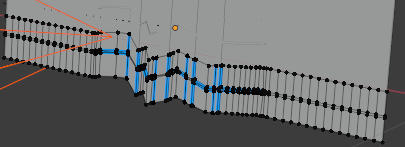
\includegraphics{images/tire_pattern.png}
    \caption{Tire pattern}
    \label{fig:tire_pattern}
\end{figure}

After creating the pattern we need to transform it so it resembles a tire shape. The best way to do this is transform the pattern model using a bezier curve (figure \ref{fig:tire_curve}). 
\begin{figure}[H]
    \centering
    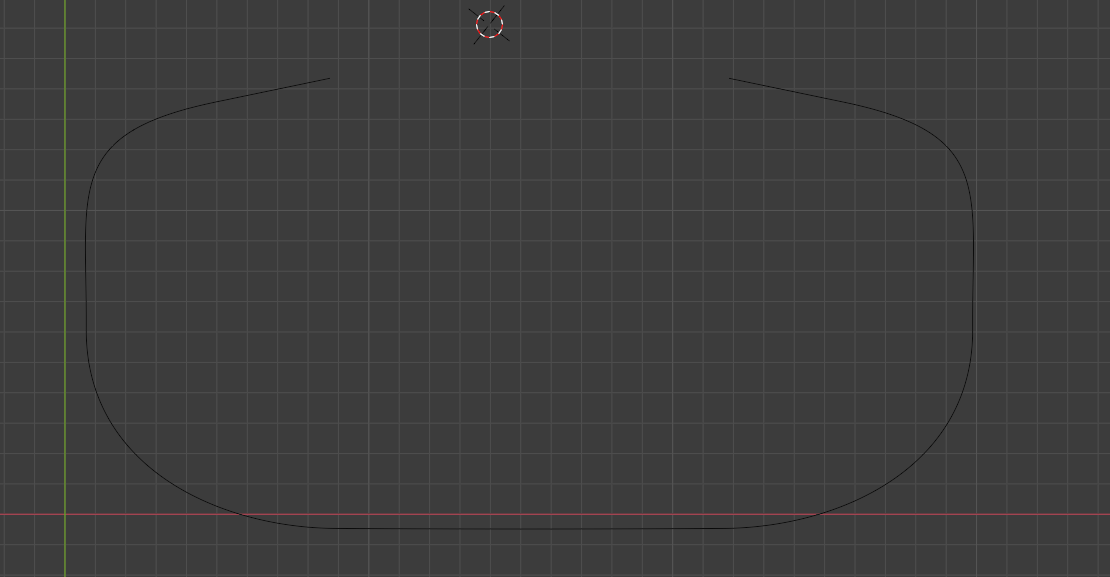
\includegraphics{images/tire_curve.png}
    \caption{Tire curve}
    \label{fig:tire_curve}
\end{figure}
And then wrap the result around a circle while adding Array modifier to the original pattern model. This results in a tire. The final step is to fit the tire to the rim we created earlier.

\begin{figure}[H]
    \centering
    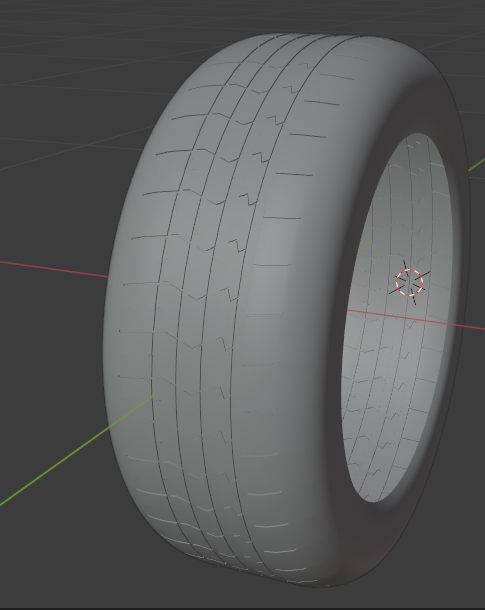
\includegraphics{images/tire_done.png}
    \caption{Finished tire}
    \label{fig:finished_tire}
\end{figure}

The finished rim with tire can be combined into a single object and used for instancing wheels for the car. The car obviously needs lights as well, but those are fairly simple to do.

Next up we need to add material properties to parts of the car. The body of the car uses Principled BSDF with hightened metallic property and so does the wheel rim. Car's windows use a mix of Diffuse and Glossy BSDF and lights use Emissive ones.

Next up is the road. Firstly I created the randomized area around the road itself. I started with a plane and subdivided it into small parts. Then I randomly selected some vertices (figure \ref{fig:rand_vert}) and moved them using randomized proportional editing on the Z axis.

\begin{figure}[H]
    \centering
    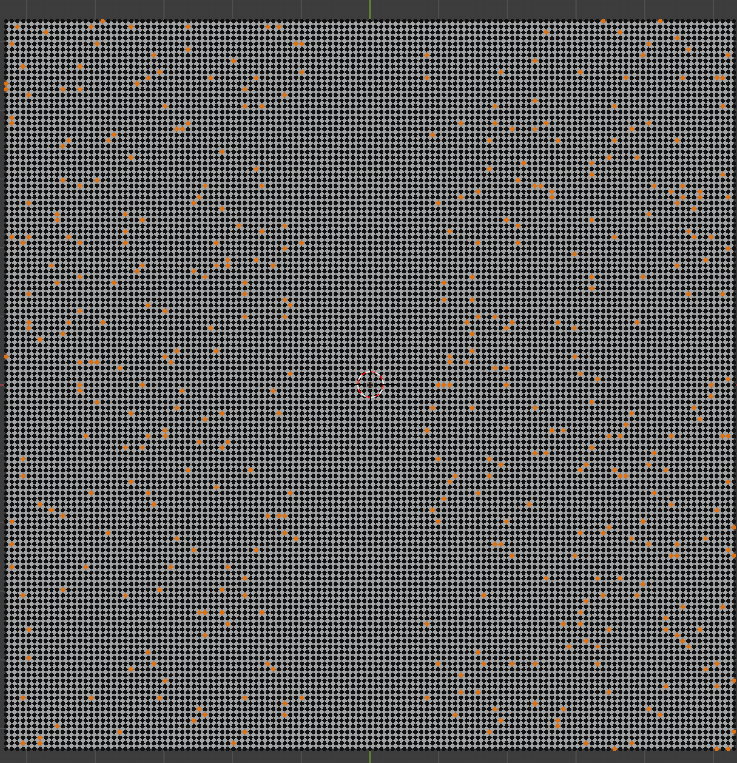
\includegraphics{images/rand_vert.png}
    \caption{Vertices for landscape}
    \label{fig:rand_vert}
\end{figure}

After moving the vertices I created a duplicate of this area and applied Wireframe modifier to it. Thanks to this there is no need to create a texture for this area, which would be unnecessarily complicated. The duplicate needs to have an Emissive shader applied to it to provide the desired effect.

\begin{figure}[H]
    \centering
    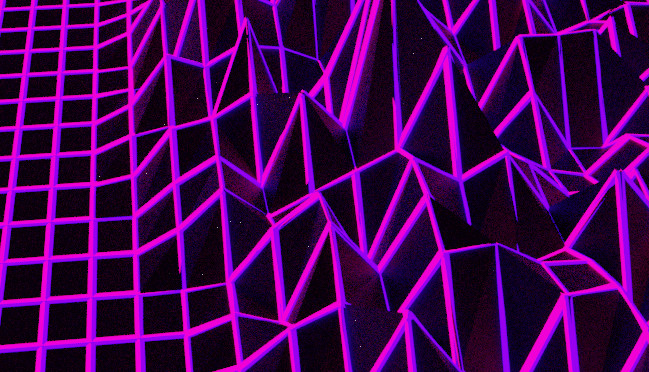
\includegraphics{images/rand_grid.jpg}
    \caption{Emissive wireframe}
    \label{fig:rand_grid}
\end{figure}

Thanks to not selecting any vertices in the middle of the area we have some space ready for an actual road. The road is quite a simple model with some emissive decorations which are repeated using Array modifier.
\begin{figure}[H]
    \centering
    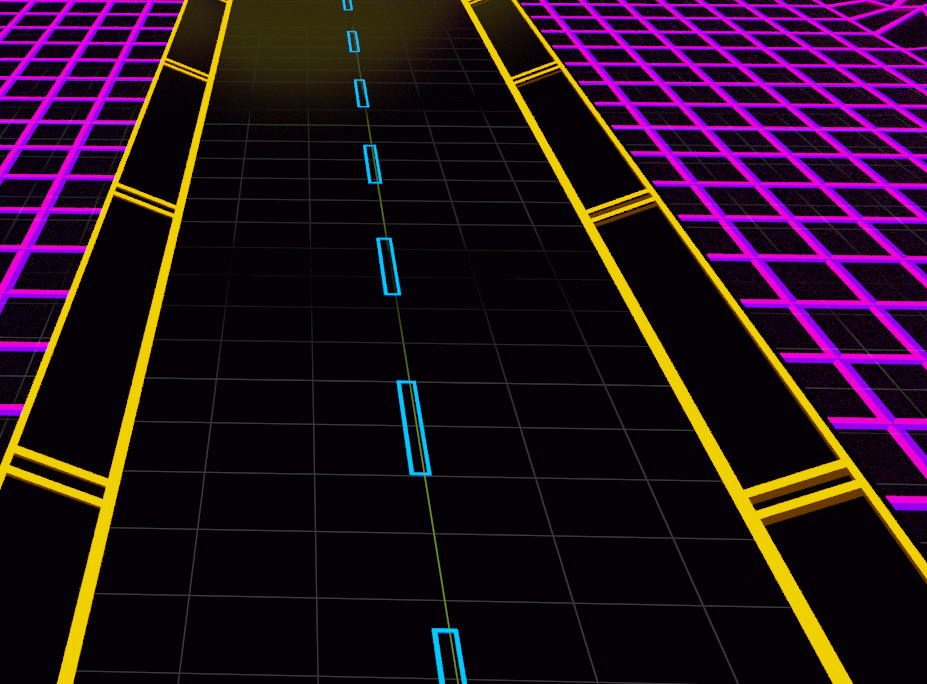
\includegraphics{images/road.jpg}
    \caption{Road}
    \label{fig:road}
\end{figure}

The final interesting part is a neon city, which is an area within the scene where multiple buildings are instanced to give an illusion of far away city. These models are really simple and the neon effect on them is done in the same way as in the landscape.
\begin{figure}[H]
    \centering
    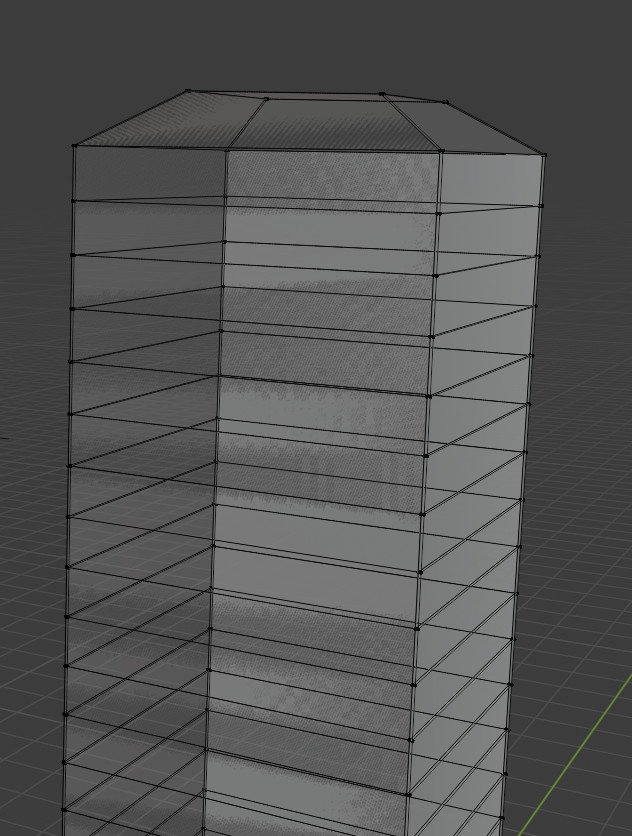
\includegraphics{images/building_wire.jpg}
    \caption{Building example}
    \label{fig:building_example}
\end{figure}



\section{Results}
This section shows models and renders of this project. Blender project files can be downloaded from \url{https://mega.nz/file/QwsFnKQY#4R2TyAcwV3gUDh2bpX7x6frqpCSw1AGGbXBuitvUlyo}.

\subsection{Car}
Model of a car is divided into several parts. The first part is the car's body and windows.
\begin{figure}[H]
    \centering
    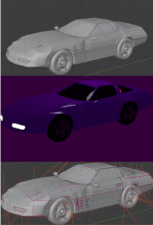
\includegraphics{images/car_render_small.png}
    \caption{Car model}
    \label{fig:car_model}
\end{figure}

Another part are lights, for which there is no necessity to showcase here, because they are very simple shames. The last fairly complex part are tires.
\begin{figure}[H]
    \centering
    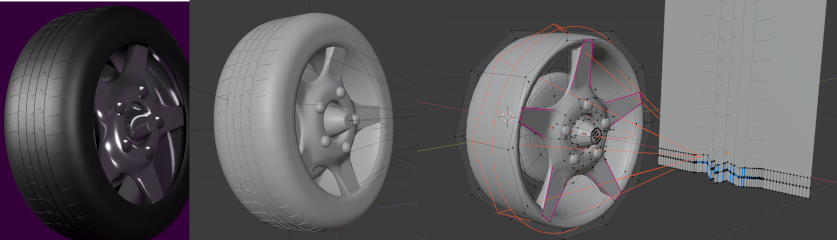
\includegraphics{images/tires_render_small.png}
    \caption{Tire model}
    \label{fig:tire_model}
\end{figure}

\subsection{Landscape}
Landscape is divided into 3 separate parts. First of them is the road and randomly generated area around it.
\begin{figure}[H]
    \centering
    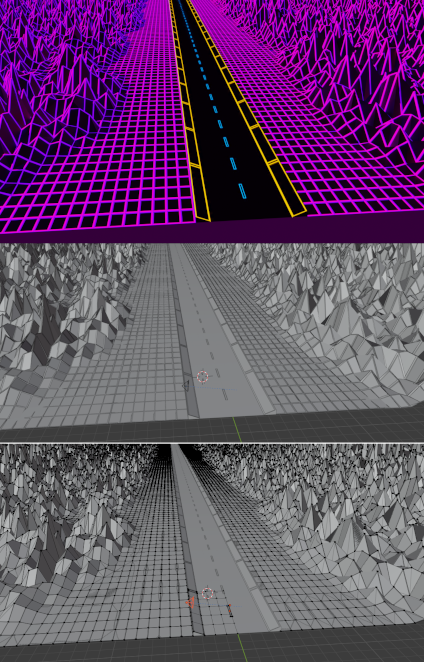
\includegraphics[scale=1.3]{images/road_render_small.png}
    \caption{Road model}
    \label{fig:road_model}
\end{figure}

Another one are buildings and the last one is a skybox texture.

\begin{figure}[H]
    \centering
    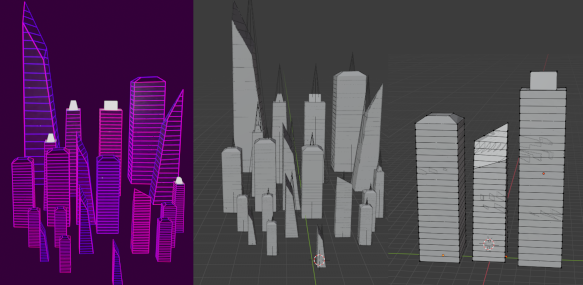
\includegraphics[scale=1.3]{images/buildings_render_small.png}
    \caption{City buildings}
    \label{fig:city_scene}
\end{figure}

\subsection{Composed scene}
All of the aforementioned models are combined together to create the following scene. Another result is an animation, which you may view at \url{https://www.youtube.com/watch?v=9Whg46x_1X0}.
\begin{figure}[H]
    \centering
    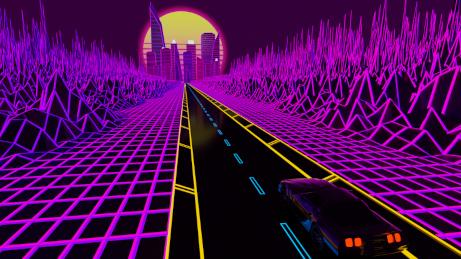
\includegraphics{images/render_small.png}
    \caption{Final result}
    \label{fig:final_scene}
\end{figure}

\section{Conclusion}
I am fairly content with the resulting renders. Results fit aesthetically very well to how I imagined it. Some improvements could be made in the animation are and the landscape could be made proceduraly in order to provide an option to render an 'infinite' animation.

\newpage
\listoffigures

\bibliographystyle{plain}
\begin{flushleft}
  \bibliography{references}
\end{flushleft}

\end{document}

